\section{Complete parameter-study context}
\label{app:parameter}
The fixed-topology study and V2 use different sources, horizons, design spaces
and losses. They are retained because they answer different questions, not
combined into one leaderboard. Table~\ref{tab:integrated-parameter-designs}
shows both distinct designs, rather than imply that three objective names
produce three different institutions.

\begin{table}[ht]\centering\small
\caption{Full frozen parameter settings. Topic and burden independently select
the right-hand design. Funding application cost is fixed at 1 in both.}
\label{tab:integrated-parameter-designs}
\begin{tabular}{lrr}\toprule
Parameter & Participation-selected & Topic/burden-selected\\\midrule
Acceptance rate & .496777 & .113159\\
Funding application cost &1&1\\
Funding slot fraction &.390677&.327413\\
Resubmission cost &12.8905&16.3863\\
Review policy &persona&standardized\\
Reviewer capacity &8&2\\
Reviewer matching &topic&random\\
Reviews per paper &3&4\\\bottomrule
\end{tabular}\end{table}

The retained intervals are exact nonparametric percentile bootstrap intervals
for the complete LossSpec aggregate over the five declared evaluation seeds.
They are not confidence guarantees for a different source or a broader model
population. All nine paired loss-contrast intervals include zero. Two labels
share a design but have separate stochastic held-out trajectories; comparing
them as if they were distinct institutions would exaggerate diversity.

\begin{figure}[p]\centering
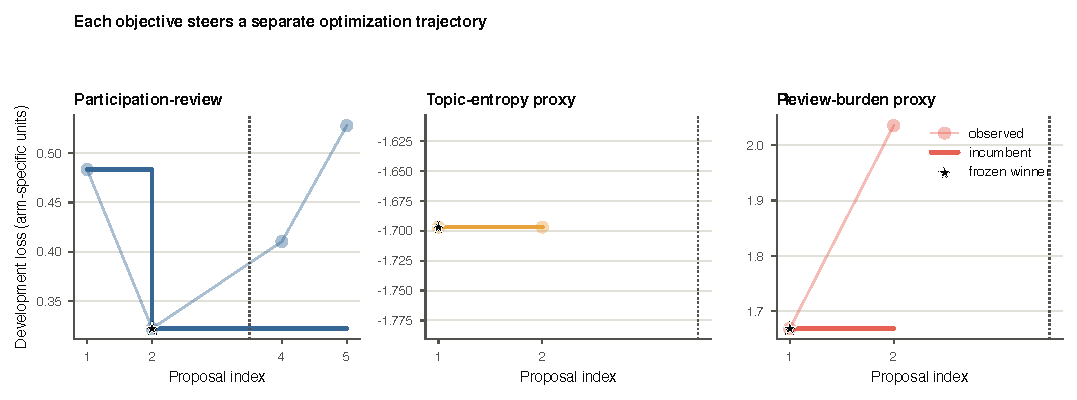
\includegraphics[width=\linewidth,height=.78\textheight,keepaspectratio]{generated/metric-conditioned/figures/metric-conditioned-objective-trajectories.pdf}
\caption{\textbf{Complete parameter-study development paths.} Three fixed
objectives, five candidates per arm and common development conditions.
Technical nulls do not become numeric penalties. Stars are frozen selections;
these are not additional held-out results or an optimizer comparison.}
\label{fig:integrated-parameter-paths}
\end{figure}

Declared gaming flags in that study are diagnostic alerts, not invalidity or
adoption vetoes. They do not override the loss. Recorded attempt runtime is
at least 52.35 h across that historical study, with one interrupted attempt's
wall time unknown; it is neither the later V2 runtime nor new compute for
this integrated manuscript. Logical rows, physical executions, adopted
trajectories and retries remain separate in the original paper slice.

\section{Complete structural case tables and interpretation}
\label{app:structural}
\begin{table}[h]\centering\small
\caption{All eight V8 structural-case outcomes. Graph is nodes/edges.
$U=3.25A-Q+0.05R$ differs from V2's $C$. Each row is a development execution;
cross-scores reuse its checkpoint. Values are display-rounded only.}
\label{tab:integrated-v8-all}
\begin{tabular}{llrrrrrr}\toprule
Arm & Generation/draw & Graph & $A$ & $Q$ & $R$ & $T$ & $U$\\\midrule
Throughput&G0/0&16/22&9&29&27&-9&1.6000\\
&G0/1&16/22&9&29&27&-9&1.6000\\
&G1/0&17/24&10&31.3333&30&-10&2.6667\\
&G1/1&16/22&10&33.6667&30&-10&.3333\\\addlinespace
Utility&G0/0&16/22&0&0&0&0&0\\
&G0/1&16/22&0&0&0&0&0\\
&G1/0&18/24&1&3.6667&18&-1&.4833\\
&G1/1&18/24&1&3.6667&18&-1&.4833\\\bottomrule
\end{tabular}\end{table}

An initial V8 authoring attempt fails before native inference because its
parent normalization does not match the exact saved request. That zero-world
failure remains in provenance, not as a fabricated scientific loss or a
successful attempt. The separately declared corrected-file workflow does not
replace an unsuccessful native trajectory. External authors may inspect their
own source and traces, richer information than a scalar-only oracle.

\begin{table}[h]\centering\small
\caption{All six V12 free-redesign observations, including the worse clinic
revision and return to its actual incumbent parent. Repetition is not new
invention; $Q$ uses original review means.}
\label{tab:integrated-v12-all}
\begin{tabular}{llrrrrrr}\toprule
Arm & Generation & Graph & $A$ & $Q$ & $R$ & $T$ & $U$\\\midrule
Throughput&G0&17/25&10&$95/3$&30&-10&$7/3$\\
&G1&17/25&10&$95/3$&30&-10&$7/3$\\
&G2&17/25&10&$95/3$&30&-10&$7/3$\\\addlinespace
Utility&G0&16/22&3&$32/3$&15&-3&$-1/6$\\
&G1&17/24&1&4&15&-1&0\\
&G2&16/22&3&$32/3$&15&-3&$-1/6$\\\bottomrule
\end{tabular}\end{table}

In V12, 32 source/context/result executions join committed native events;
throughput's10 amendments per world match generated outputs and annual
project state. Utility G1 emits two year 1 amendments and no additional year 2
clinic amendment. The historical code ABI does not retain a fully bound
upstream plan, so a stronger complete applied-plan hash cannot be reconstructed
for that slice. V13 prospectively records the full upstream plan and ordered
commands, enabling the stronger join. Later provenance improvements do not
retroactively repair old records.

For V13, actual eligible reviewer identities pass through a typed routing
capability to the original review prompt/model/parser. The source chooses a
subset of tasks, including none; the host does not choose favorable scores.
Original eligibility/COI and identity legality remain explicit native semantics.
A zero-review rule must author its own compatible selection consumer. The
new G1 ranking uses prior reviews to predict task desirability, not to replace
actual reviewer evidence in the measurement.

\FloatBarrier
\section{Gradient assumptions, diagnostics and complete followups}
\label{app:gradient}
\subsection{What each derivative covers}
For a categorical choice with logits $\alpha $, the sampled score is the
one-hot choice minus its probability vector. For a Gaussian latent with mean
$\mu $ and fixed scale $\sigma $, the mean score is $(z-\mu)/\sigma^2$.
These derivatives concern the retained sampling law. A fixed sigmoid mapping
the latent to a bounded cutoff does not require a native world derivative in
the LR estimator. Replacing the sampling law, truncating its support without
accounting, or changing source semantics changes the estimator's target.

Leave-one-out baselines rely on conditional independence of the other design
draws; they are not a license to reuse arbitrary correlated outcomes as a
baseline. Controls in Eq.~\eqref{eq:integrated-control} are fixed from eligible
prior history for the current scored batch. Their expectation correction
must be computed for the same distribution. If the world's conditional law
depends on $\theta $ beyond the sampled executable design, the stated simple
score identity is incomplete. Missing technical outcomes and adaptively
selected histories require their own estimand analysis.

The local response representation takes a different route: it approximates
sensitivities inside the native path. A faithful hard replay verifies value
accounting, not the correctness of its soft derivative. A parameter disconnected
inside the explicitly represented subgraph can have derivative zero there;
unknown external researcher/host responses must remain unknown. Neither LR
nor the response operator differentiates arbitrary LLM source invention.

\begin{table}[h]\centering\small
\caption{All V9 coupled-history endpoints. C: calibration; U: unused coordinate;
G: frozen gradient proposal. The proposal at .50 is an exact no-op at stored
precision. The better observed .80 is not substituted for it.}
\label{tab:integrated-v9-all}
\begin{tabular}{lrrrrrr}\toprule
Role &$\theta $&$A$&$Q$&$R$&Native $U$&Predicted $U$\\\midrule
C0&.20&0&0&18&.9000&.9000\\
C1&.50&0&0&18&.9000&.9000\\
C2&.80&1&$10/3$&18&.8167&.8167\\
U0&.35&0&0&18&.9000&.9000\\
U1&.65&0&0&18&.9000&.8168\\
G&.50&0&0&18&.9000&.9000\\\bottomrule
\end{tabular}\end{table}

\begin{figure}[p]\centering
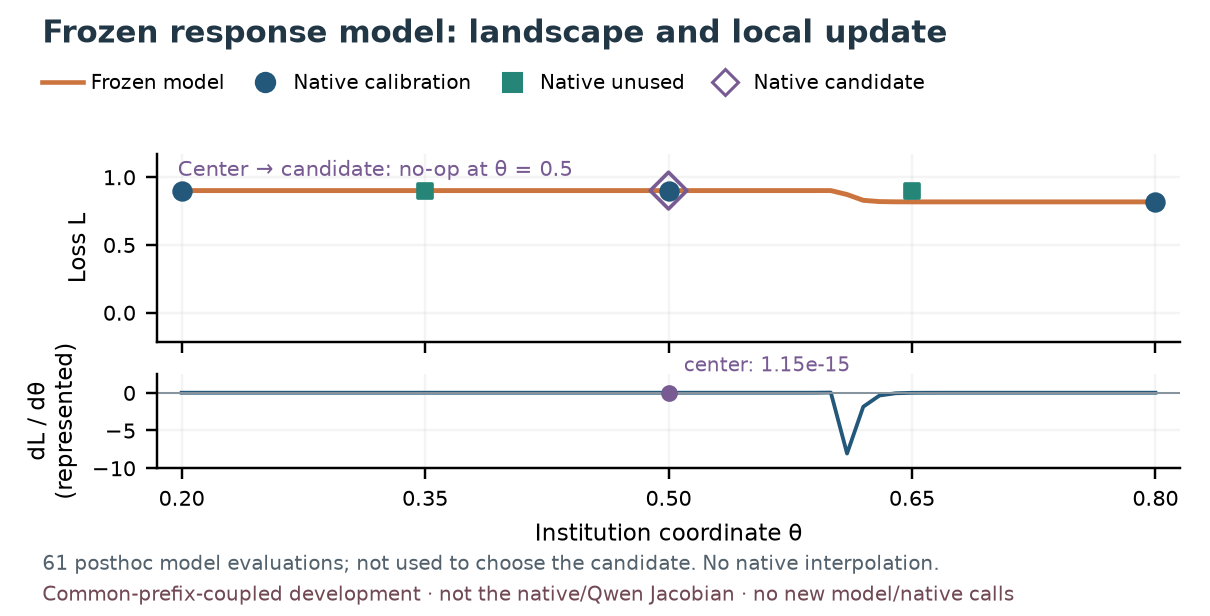
\includegraphics[width=\linewidth,height=.78\textheight,keepaspectratio]{figures/native-qwen-response-v9-a3-landscape.png}
\caption{\textbf{Frozen represented landscape and actual native endpoints.}
The plotted model evaluations are offline diagnostics, not new Qwen calls.
Calibration fit does not imply unused-coordinate or finite-path fidelity.
The precommitted gradient candidate remains the center rather than the known
lower calibration endpoint.}
\label{fig:integrated-response-landscape}
\end{figure}

\begin{table}[h]\centering\small
\caption{Offline temperature diagnosis at $\theta=.5$ on the same historical
calibration data. These are not four native experiments or prospective
temperature selection using future success.}
\label{tab:integrated-temperature}
\begin{tabular}{rrr}\toprule
Temperature & Center represented derivative & Calibration-loss RMSE\\\midrule
1&$-.24092$&.52717\\
.2&$-.09426$&.32974\\
.05&$+.01156$&.01522\\
.01&$1.15\times 10^{-15}$&$1.16\times 10^{-5}$\\\bottomrule
\end{tabular}\end{table}

The V10 gradient steps use a fixed temperature schedule $(1,.2,.05)$ and
$\theta_{k+1}=\operatorname{clip}_{[.2,.8]}[\theta_k+
\operatorname{clip}_{[-.1,.1]}(-.5\widehat g_k)]$.
They refit on only the three shared calibration endpoints and their own earlier
completed endpoints. The black-box policy instead refines the widest interval
adjacent to its observed incumbent, choosing the lower interval on ties.
Each arm's new losses are $(.9, 49/60, 49/60)$; neither beats the shared historical
best. Their six forwards contain 504 logical replies, 318 prefix replays and 186
new calls; support from shared historical calibration is counted once, not once
per method or as six independent societies.

\subsection{Score/control measurements and the previously missing forward}
V11's two arms each have four native losses $(.7833333, 1.2, 1.2, 1.2)$.
The first draw has $A=1,Q=11/3,R=24$; each remaining draw has $A=Q=0,R=24$.
The G0 score step changes Gaussian mean from 0 to $-.0407768$ and logits to
$[-.0495833,.0495833]$ before G1. The final prior-control estimate has mean
gradient $.742395$ and logit gradient $[.109754,-.109754]$; plain LR on the same
batch gives $.945250$ and $[-.570274,.570274]$. These single noisy estimates
are not empirical variance measurements.

The saved final mean $-.1150163$ and logits $[-.0605587,.0605587]$ are not
reevaluated within V11. Table~\ref{tab:integrated-control-forward} records the
separate complete two-world followup, not a retroactive extra V11 generation.
Historical outcomes are provenance, not a randomized concurrent control.

\begin{table}[h]\centering\small
\caption{Complete fresh followup of the exact saved V11 proposal. The bounded
executable cutoff differs from its Gaussian latent. Lower is better under the
same $U$, but two draws do not estimate comparative expected improvement.}
\label{tab:integrated-control-forward}
\begin{tabular}{lrrrrrr}\toprule
Aggregation&Cutoff&$A$&$Q$&$R$&$U$&Fresh replies\\\midrule
Minimum&3.549508&0&0&21&1.05&91\\
Mean&3.080488&2&7&21&.55&89\\\bottomrule
\end{tabular}\end{table}

\FloatBarrier
\section{V2 all-candidate cross-scores and failure accounting}
\label{app:failures}
The two matrices retain all 60 scheduled rows per primary objective, including
three histories and four generations for each method. G/X marks denote
generation/execution nulls, not zeros. Full-precision values, raw metric
components and missingness remain in the numerical JSON/CSV; display rounding
never affects selection. Loss scales are independent and not combined.

\begin{figure}[p]\centering
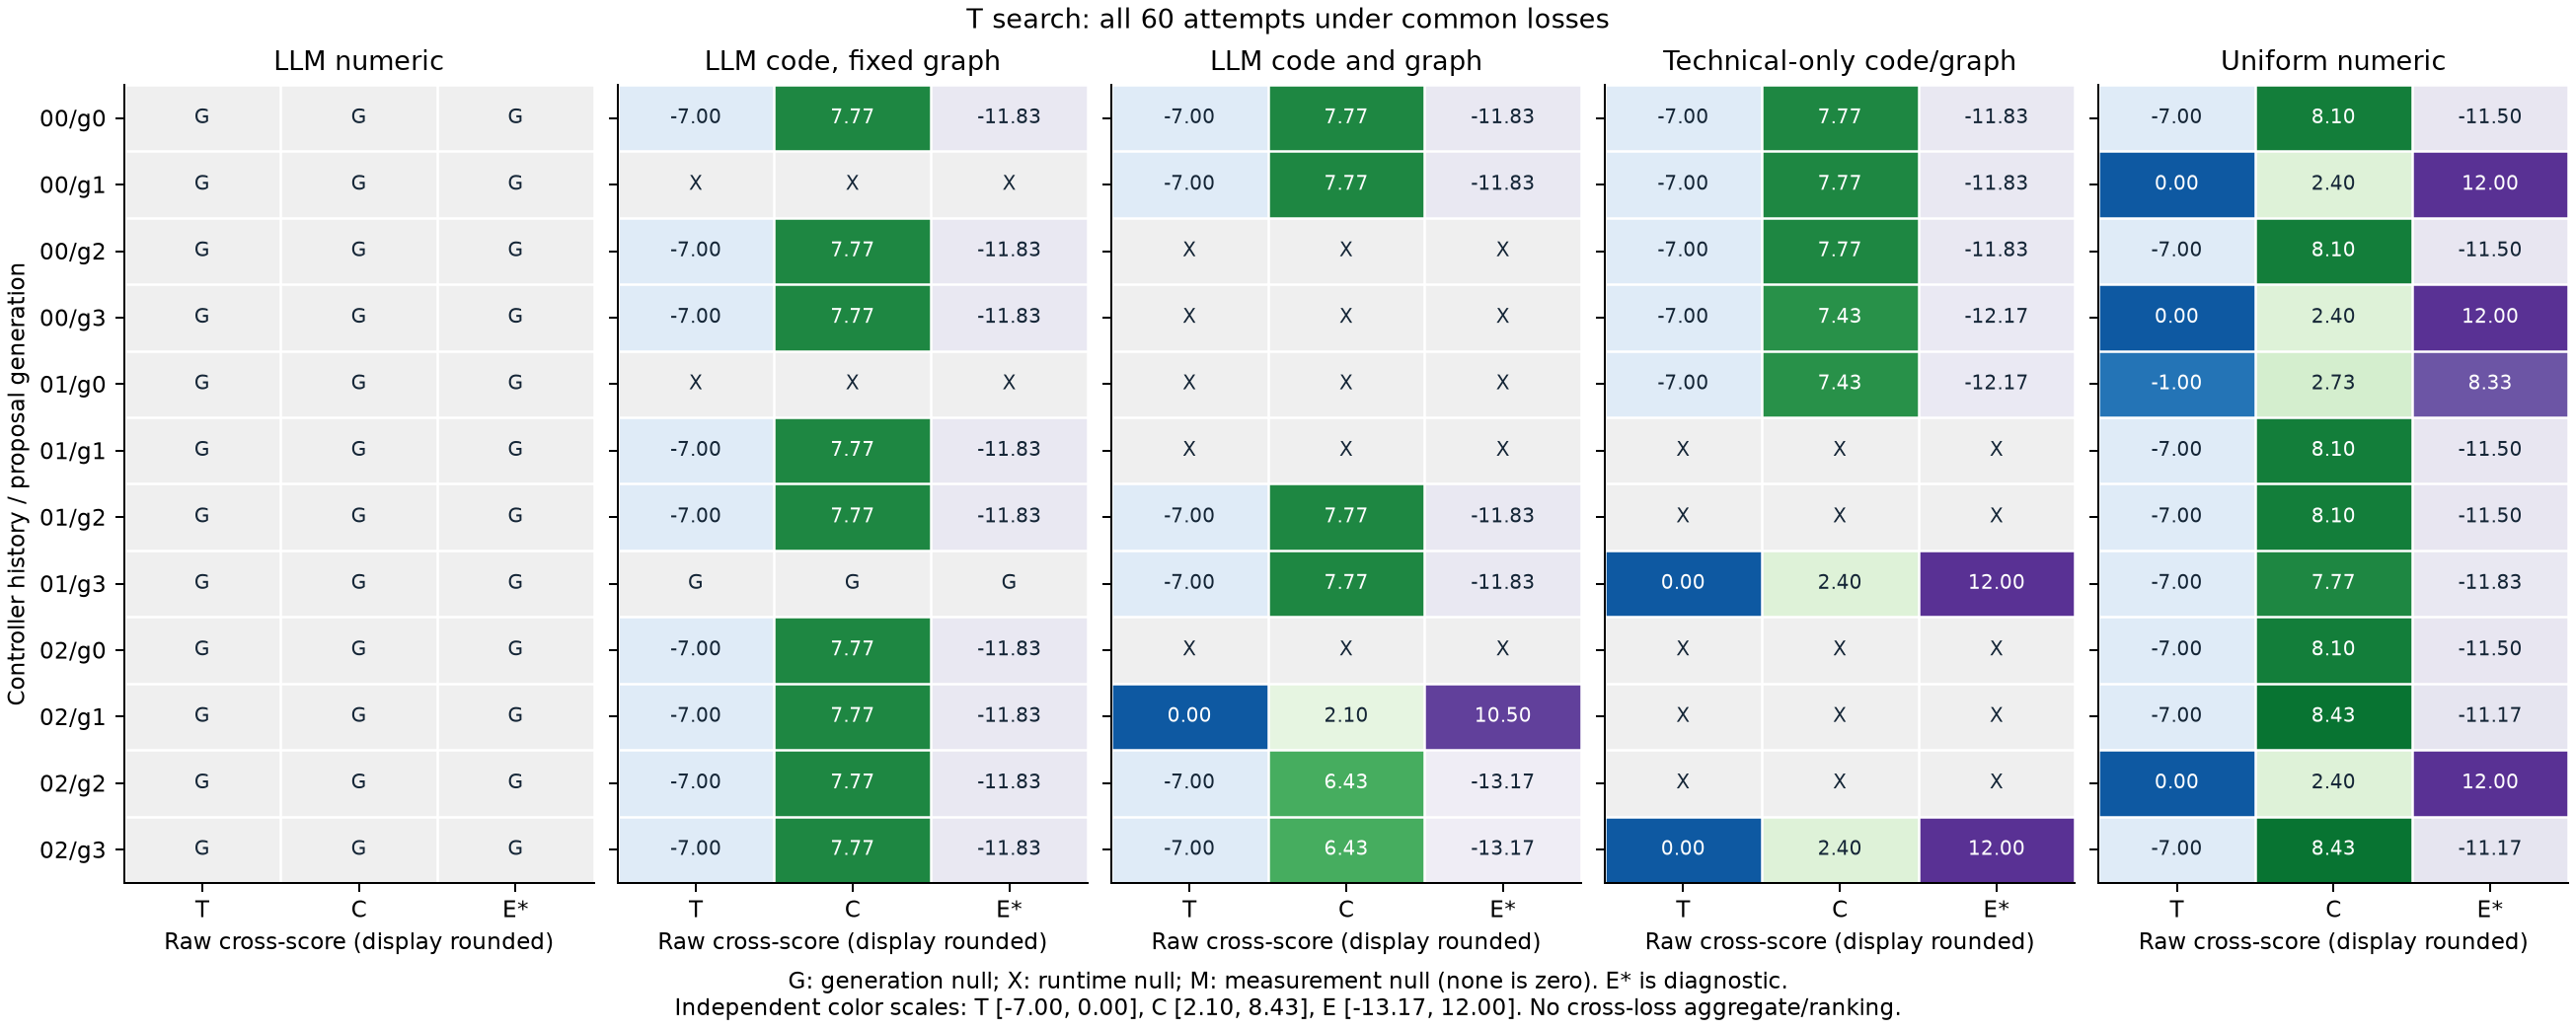
\includegraphics[width=\linewidth,height=.79\textheight,keepaspectratio]{generated/native-design-v2-supplement/all-cross-scores-throughput.png}
\caption{\textbf{Every V2 throughput-arm attempt under T/C/E.} These are
development cross-scores, not E-optimized selections or extra worlds. A favorable
E observation in a T arm is not relabeled an E-search result.}
\label{fig:integrated-all-t}
\end{figure}
\begin{figure}[p]\centering
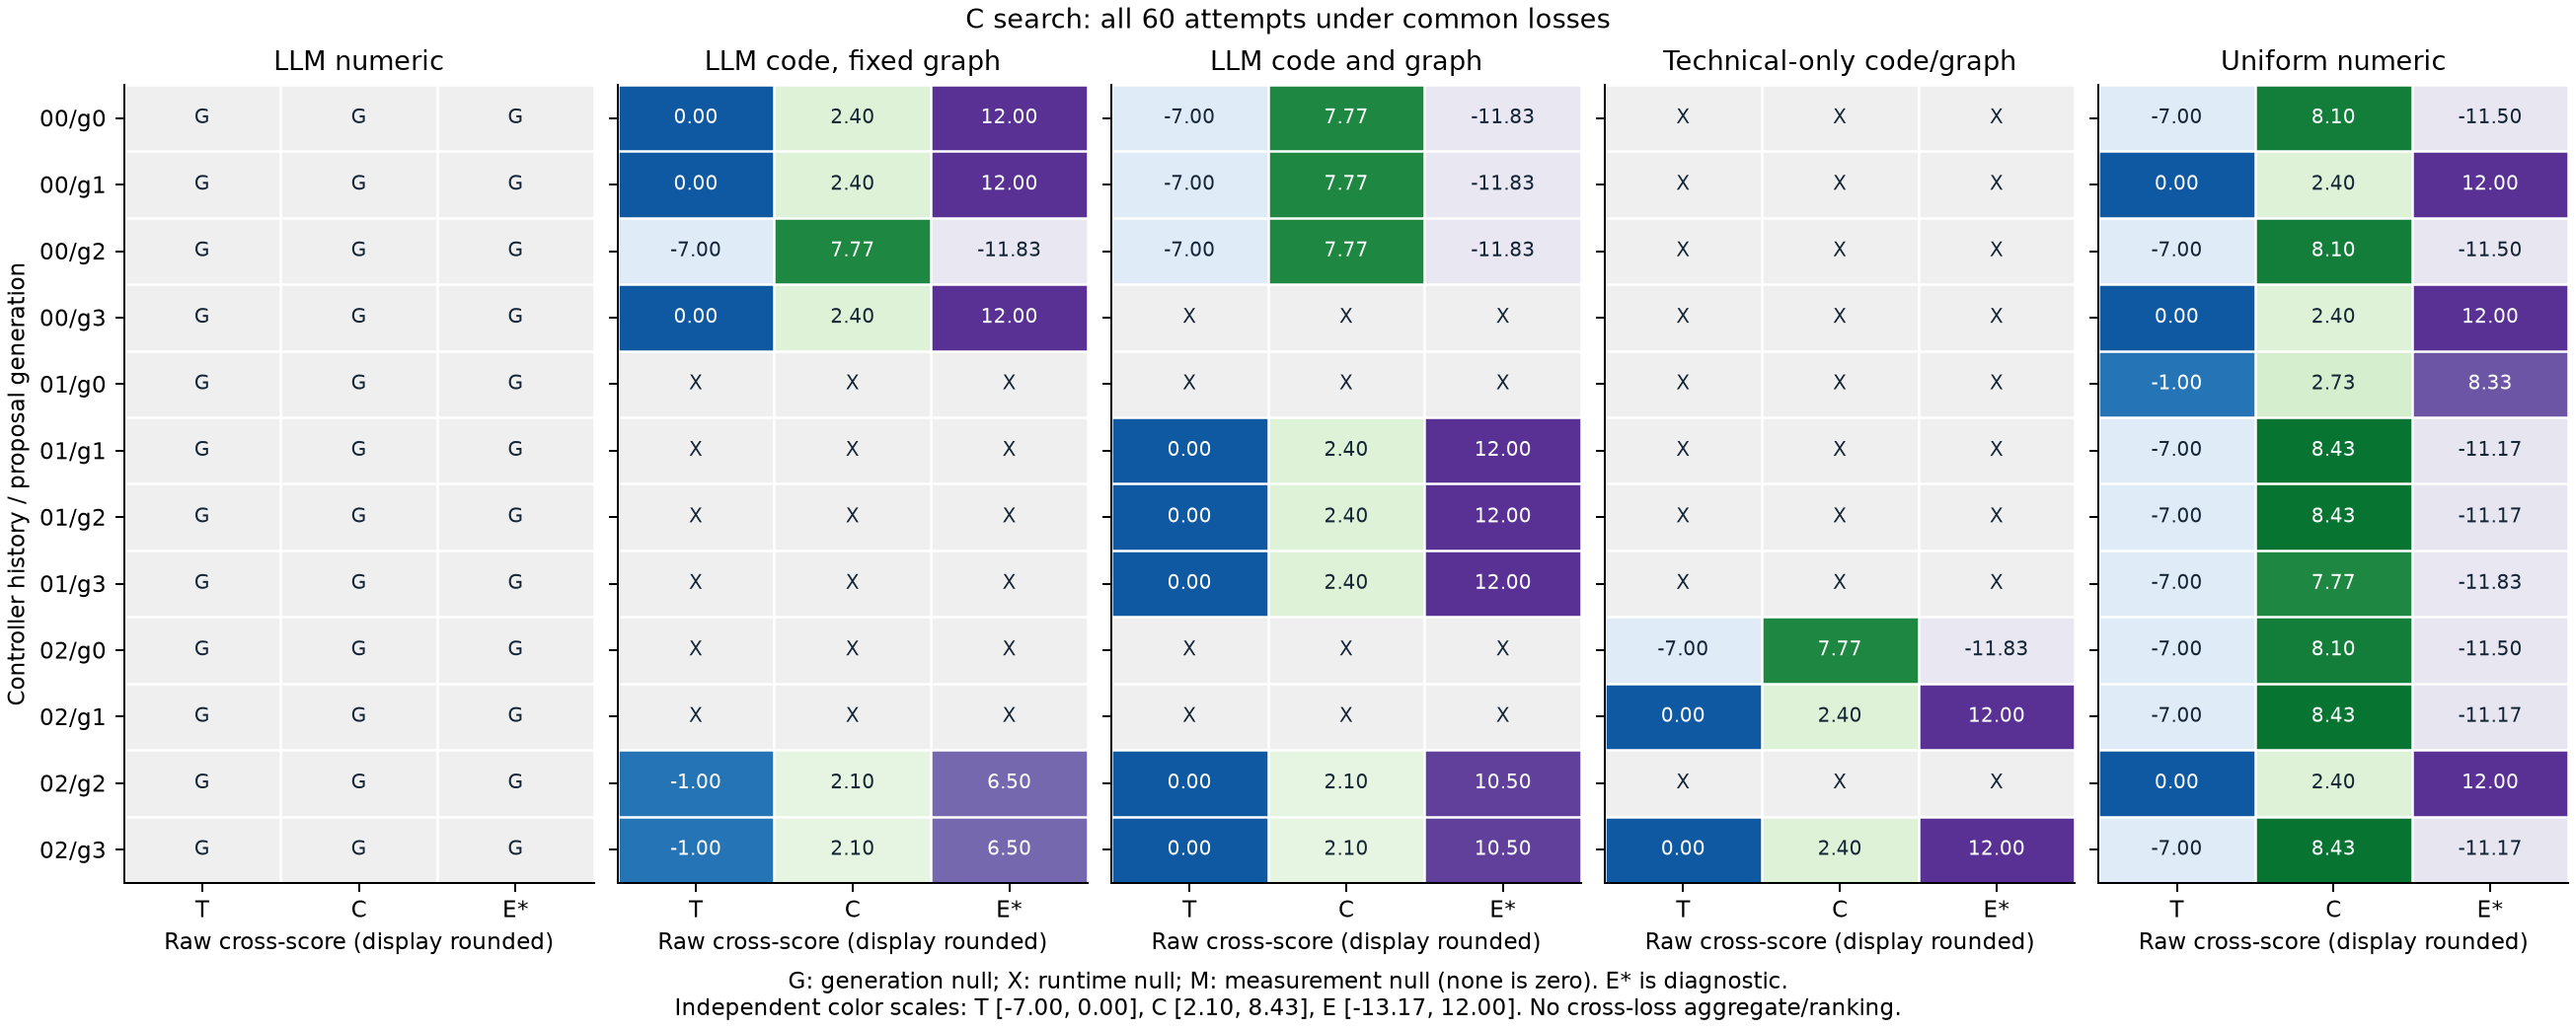
\includegraphics[width=\linewidth,height=.79\textheight,keepaspectratio]{generated/native-design-v2-supplement/all-cross-scores-selective.png}
\caption{\textbf{Every V2 C-arm attempt under T/C/E.} All failed attempts,
initial selections, ties and worse generations remain; there is no best-run-only
or successful-proposal-only reporting.}
\label{fig:integrated-all-c}
\end{figure}

The 31 execution failures comprise scalar-shape misuse 12, world-envelope errors 7,
decision-identity coverage 6, missing outputs 4, an extra output 1 and invalid
decision/score/reference 1. These are literal observed categories, not isolated
causes of designer cognition. The 25 generation-null slots exhaust the declared
action budget without valid explicit finish. A final provider envelope or
HTTP 200 is not necessarily a submitted executable institution.

The distinction between permission and use is also numerical: 40 of 64 completed
specifications change selection source; existing parameter-change row counts
overlap (bias 26, memory cost 24, threshold array 25, process count 20, router
threshold 24). No declared node/wiring/ABI/state/schedule changes are observed.
String/source identity, AST identity and arbitrary-input behavioral equivalence
are separate notions, none a hidden novelty gate.

\section{V2 costs, resources and separate longer horizon}
\label{app:costs}
\begin{table}[h]\centering\small
\caption{Search-only V2 components, pooled across three four-slot histories.
Designer seconds are host model-call time, not end-to-end wall or total compute.
Scientist replies include partial worlds. Zero author calls in uniform sampling
does not make native evaluation free.}
\label{tab:integrated-method-costs}
\begin{tabular}{llrrrrr}\toprule
Loss&Method&Complete/12&Author calls&Author s&Scientist replies&World dirs\\\midrule
T&Numeric LLM&0&192&2497.2&0&0\\
T&Code/fixed&9&172&2219.1&859&11\\
T&Code/graph&7&168&2413.4&739&12\\
T&Technical-only&7&168&2318.9&745&12\\
T&Uniform&12&0&0.0&1097&12\\\addlinespace
C&Numeric LLM&0&192&2580.9&0&0\\
C&Code/fixed&6&168&2519.7&682&12\\
C&Code/graph&8&167&2770.8&826&12\\
C&Technical-only&3&160&2361.9&459&12\\
C&Uniform&12&0&0.0&1107&12\\\bottomrule
\end{tabular}\end{table}

Search records 6514 scientist replies and 640 institution-code executions. Its 95
world directories, plus 9 fresh references and 90 physical evaluations, yield 194
response journals, not 194 completed forwards: completed forwards total 163.
Generation-null slots never dispatch a world. Proposal requests 1387 have 1385
final signals; validity/submission is checked separately.

\begin{table}[h]\centering\small
\caption{Measured V2 response-token scopes. Cached input counts are subsets,
not extra tokens. Model-load usage and total-project compute remain unknown.}
\label{tab:integrated-tokens}
\begin{tabular}{lrrrr}\toprule
Scope&Responses&Input&Cached input subset&Output\\\midrule
Scientists incl. partial worlds&16043&15547758&2976386&1473665\\
Designer proposals&1387&25969867&3102175&267057\\
Designer calibration&84&808832&22464&3819\\\bottomrule
\end{tabular}\end{table}

The 1764 auxiliary intents comprise 1387 proposal, 84 calibration and 293 role-load
intents. Loads separate 99 designer and 194 scientist contexts; their native
tokens are unreported, not zero. Native/provider/host durations overlap and
cannot be summed as project wall time. Overall writer wall is known, but exact
end-to-end per-trial wall allocation is not reconstructed from component data.
Retrieval, container orchestration, model loading, prior development and this
coding assistant's compute are not a measured project FLOP/energy/money total.

\begin{figure}[p]\centering
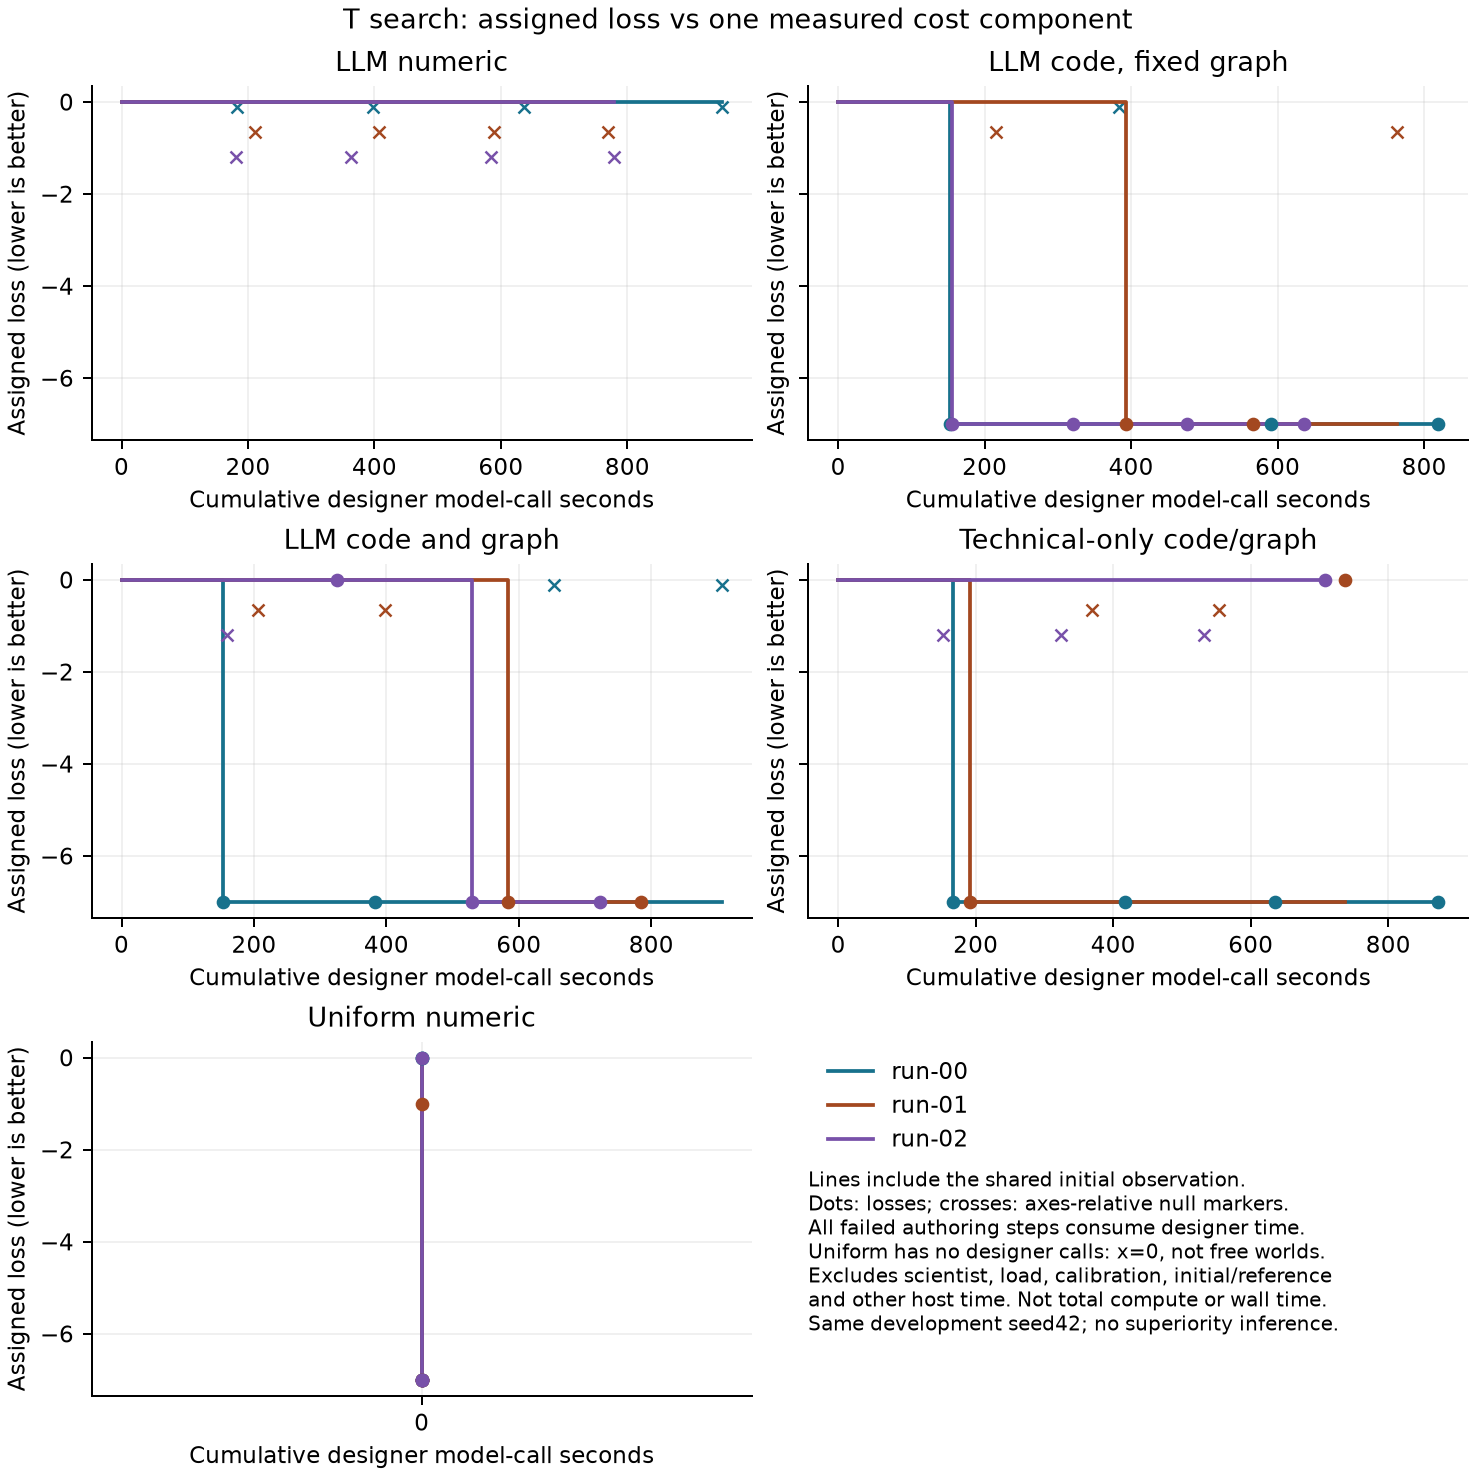
\includegraphics[width=\linewidth,height=.79\textheight,keepaspectratio]{generated/native-design-v2-supplement/designer-cost-paths-throughput.png}
\caption{\textbf{V2 T paths against cumulative designer host model-call time.}
All failed author steps are charged. Uniform is at zero designer time, not zero
world cost. Shared initial observations/calibration have separate excluded
costs; this axis is a measured component, not equal-compute superiority.}
\end{figure}
\begin{figure}[p]\centering
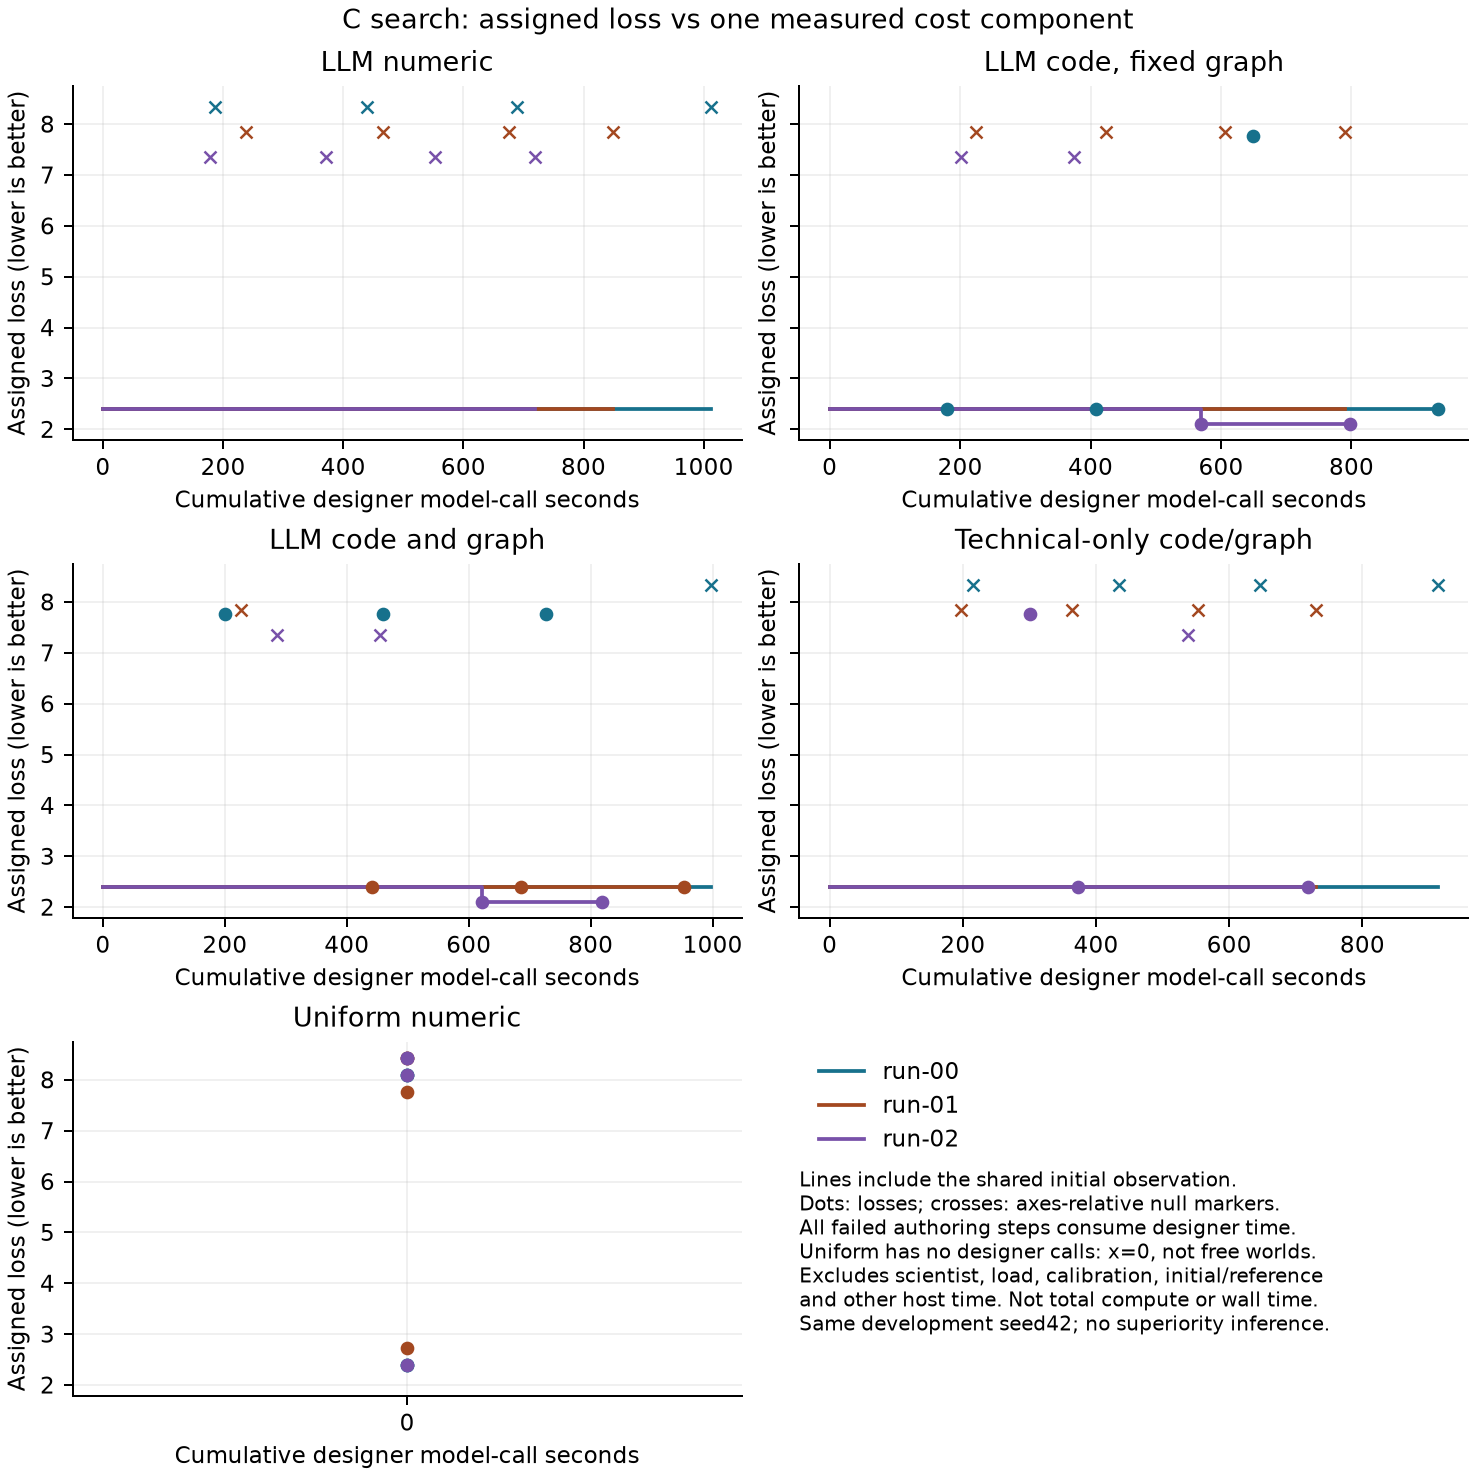
\includegraphics[width=\linewidth,height=.79\textheight,keepaspectratio]{generated/native-design-v2-supplement/designer-cost-paths-selective.png}
\caption{\textbf{V2 C paths against the same measured cost component.}
Three histories are shown without treating them as independent environments.
Missing component times would stop the cumulative axis, not be imputed as 0.}
\end{figure}

Outside metrics retain accepted decisions, original accepted peer-score sum,
review records, final original active authors, final author resources,
unreviewed acceptances, rejections and institutional-context deliveries.
Two-year resource means/ranges include initial 616(585--630),C code 627(595--640)
and T uniform 632(620--640). Descriptive overlap is not an equivalence test;
differences are not isolated causal benefits. Four-year initial 720,C code 780
and T uniform 760 remain single observations.

\begin{figure}[p]\centering
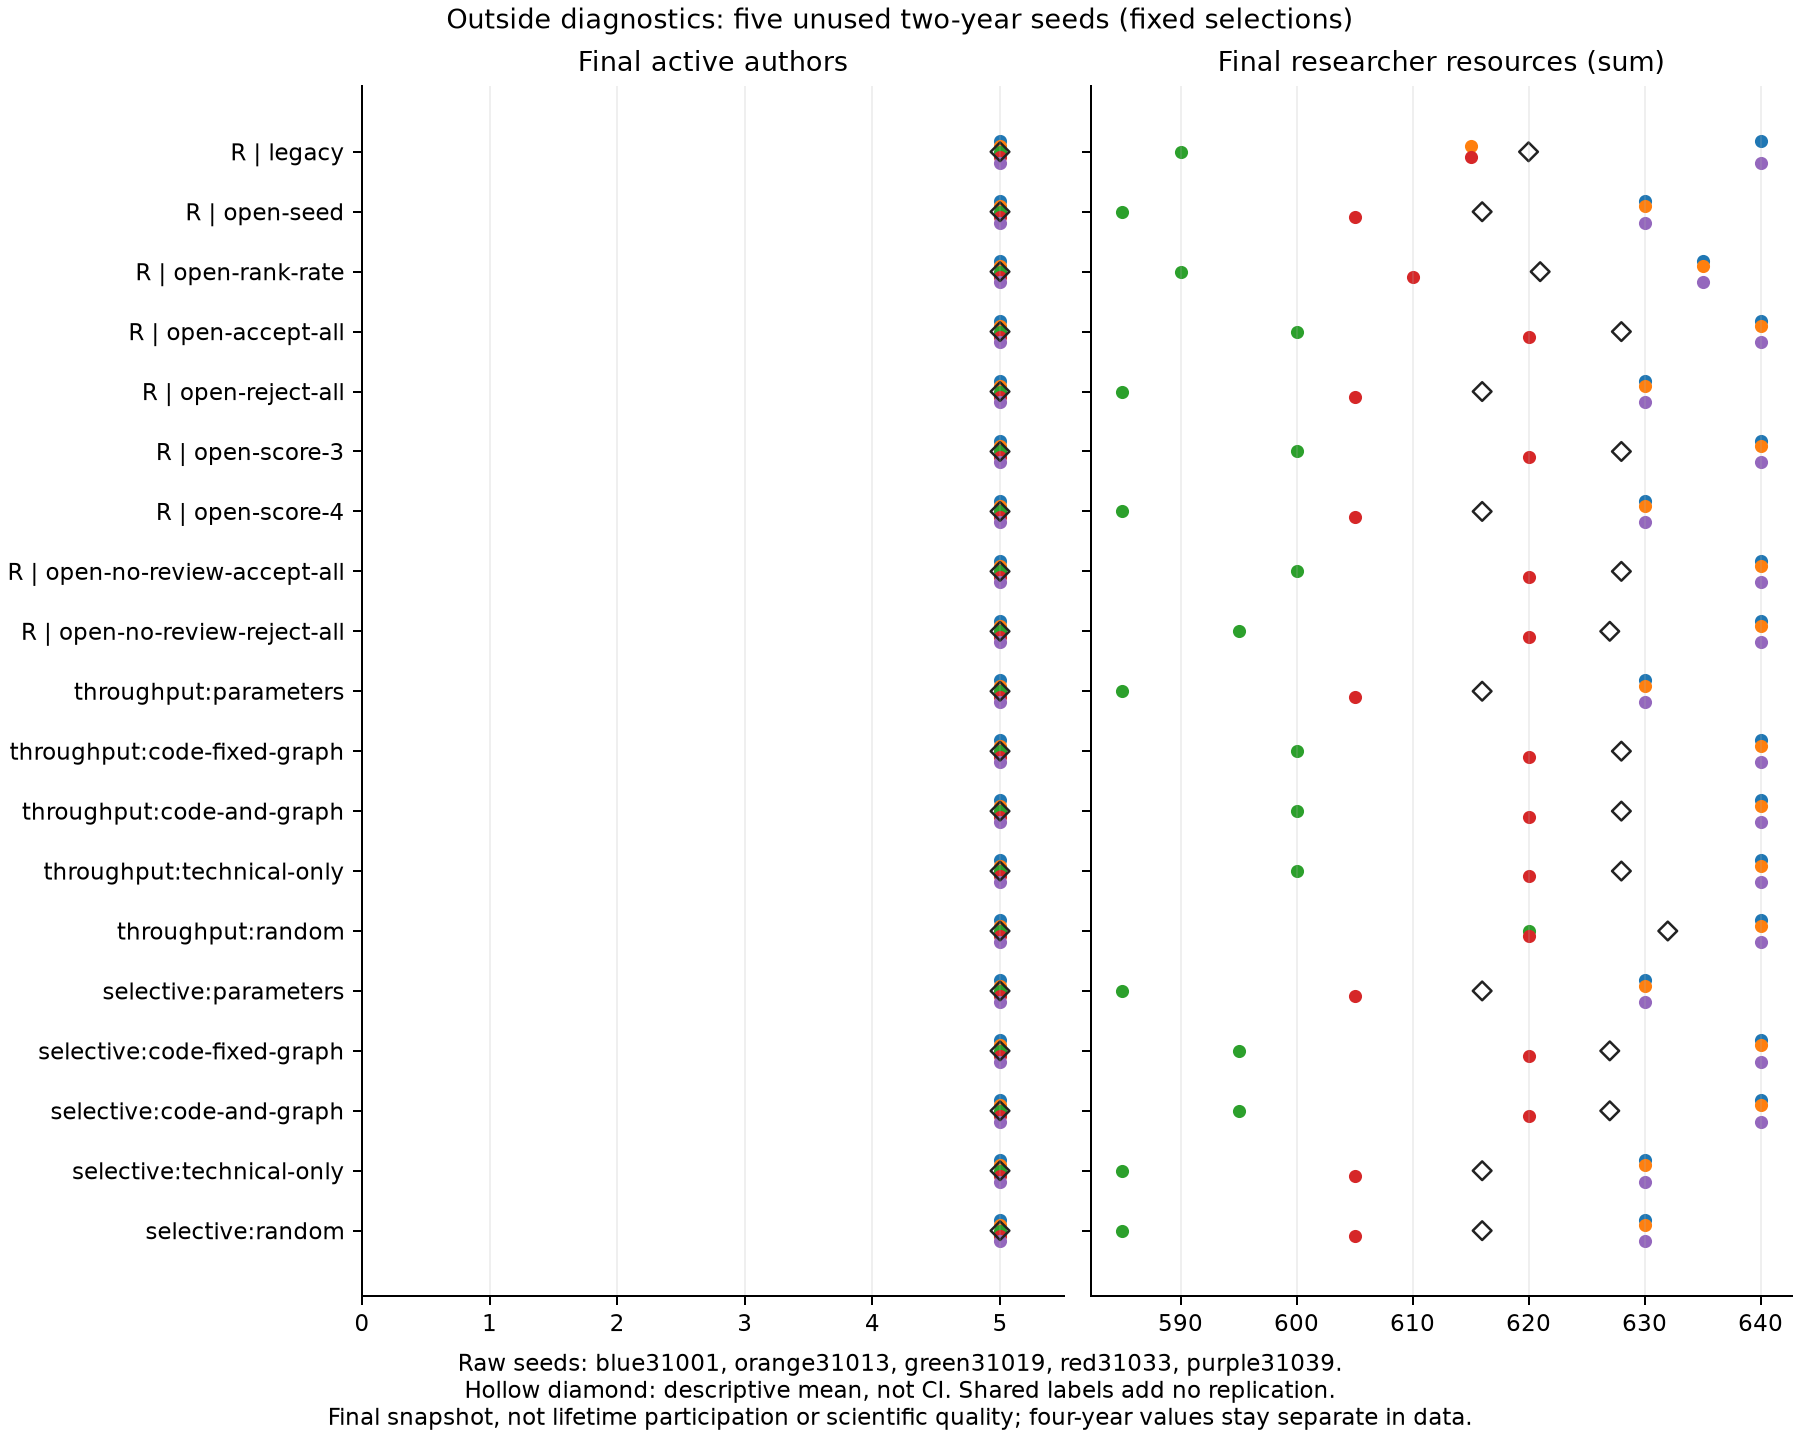
\includegraphics[width=\linewidth,height=.79\textheight,keepaspectratio]{generated/native-design-v2-supplement/outside-activity-resources-2y.png}
\caption{\textbf{V2 outside activity/resources on all selected/reference labels.}
The full 0--5 activity axis shows no final active-author separation. Five points
and descriptive means retain shared-policy identities. Native resources are
not money, welfare, scientific truth or an additional selection constraint.}
\end{figure}
\begin{figure}[p]\centering
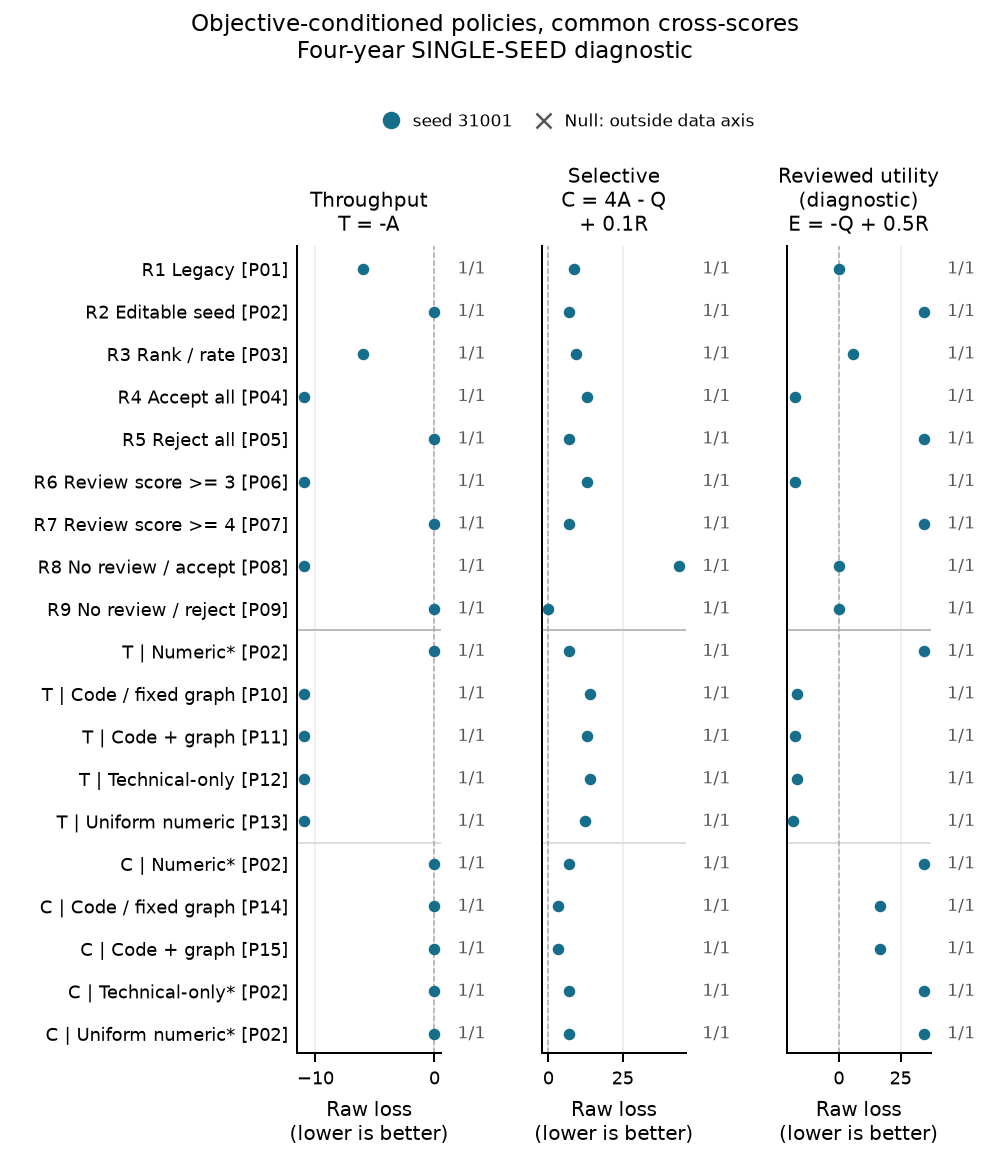
\includegraphics[width=\linewidth,height=.79\textheight,keepaspectratio]{figures/native-design-v2/cross-objective-4y.png}
\caption{\textbf{V2 separate four-year diagnostic.} One seed, no confidence
band or extra independent five-seed sample. Same labels/sharing/loss definitions
as the two-year plot. A repeated exact policy is not another observation.}
\label{fig:integrated-four-year}
\end{figure}

\FloatBarrier
\section{Fixed-record incentives versus dynamic policy optima}
For V2, freeze $N$ realized records, original reviewer means $ q_i $ (zero without
review) and review count $R$. If $ z_i\in\{0, 1\}$ only changes acceptance on those
records, then
\begin{align}
 T_{\min}^{\rm rec}&=-N,\\
 C_{\min}^{\rm rec}&=0.1R+\sum_i\min(0, 4-q_i),\\
 E_{\min}^{\rm rec}&=0.5R+\sum_i\min(0,-q_i).
\end{align}
Zero coefficients remain ties. For a full measured trajectory with $A>0$,
$C<0$ requires $Q/A>4+0.1R/A$. These elementary relations explain declared
incentives; they are not a new theorem or an optimal policy for the dynamic
world. Decisions affect later resubmissions, reviewer work, memory and resources.
The original reviews are endogenous rather than a fixed true-quality oracle.

The fixed-record projection contains 219 identities: 163 complete forwards and 56
unavailable entries. It does not execute 219 new worlds. Missing scores can make
a relaxation unavailable without invalidating a different measurable loss.
Neither this algebra nor AST/source inspection establishes equivalence on
unobserved inputs.

\section{Reproducibility, provenance and editorial scope}
\label{app:reproduction}
\subsection{Distinct execution identities}
The parameter study pins sourceZZPROTECTED 79ZZ and a simultaneous winner
sealZZPROTECTED 80ZZ. Structural V8 usesZZPROTECTED 81ZZ; free redesign
V12 usesZZPROTECTED 82ZZ; nested V13 usesZZPROTECTED 83ZZ.
The V10 method-path source isZZPROTECTED 84ZZ, and V11's native source
isZZPROTECTED 85ZZ. V2 usesZZPROTECTED 86ZZ. Full hashes, protocols and
original audit identities remain in machine-readable evidence records.
Historical reset worlds, coupled prefixes and source-equivalence bridges are
not relabeled a same-source matched experiment.

The original scientist alias isZZPROTECTED 87ZZ; the approved V2 local designer
alias isZZPROTECTED 88ZZ. Actual designer context is 40960 despite the
alias; the manifest/digest and model-load observations are retained. The upstream
revision and conversion command are unknown. Approved five HEAD-only registry
checks return advertised descriptor matches for three sampled local tensors
and two controls, with no body retrieval. They do not establish tensor contents,
all 986 descriptors, conversion provenance or fresh-machine reproducibility.

V2 uses 103107 CS 2016--2019 SciEvo records with pinned corpus/retriever binding.
The corpus is a literature-grounding substrate, not a license to redistribute
every underlying document or proof of scientific validity. Current public
model tags are not assumed equivalent to local retained weights.

\subsection{Audit and reconstruction tiers}
V2 closes with a matching normal terminal record, actual process exit 0 and
closed progress. Selection precedes first evaluation. Two read-only full audits
match byte-for-byte and verify 278 source blobs and 7038 raw files. A pinned
order-only adapter reconstructs equal-valued plan/selection mapping order lost
by sorted JSON. It preserves values, hashes, list chronology and original guards;
the unmodified frozen audit CLI is not claimed to pass. Replaying an auditor
does not create independent scientific evidence.

The exact retained closed-report archive supports numerical reconstruction:
120 statuses/ties and 90 evaluations rejoin, 462 T/C/E losses recompute from
measured $A/Q/R$ with zero residual, and 22 PNGs match the reviewed originals.
Exact auxiliary/scientist cost projections separately rebuild the full
supplement. This is not raw inference or independent replication. Paper-only
13-path subsets rebuild offline with cached tooling; rendered pages and text
match their reviewed variants, not necessarily binary PDF bytes. A cache-free
clean-machine build and fresh-model inference have not been established.

The repository exposes reproduction commands, compact JSON/CSV projections,
source-bound receipts and figure provenance. Large caches, reply databases,
corpus and model weights remain outside the publication subset. Complete
numerical projections include operational locators and are not certified
anonymous supplements. Author-name removal alone is not anonymity, rights
clearance or permission to upload. Human authors must review and accept
responsibility before an actual submission.

\subsection{What was deliberately not expanded into the scientific narrative}
Earlier local-author failures, copy controls, transport fixes and loop-retention
pilots are retained in the repository. They inform literal execution,
context-budget and completion checks. We do not count test-suite sizes or a
repaired editor protocol as a scientific discovery. S1's strong controls and
V1's eight-slot feedback pilot motivated V2 but are not pooled with its fresh
references. Numerical miniature/unit worlds verify implementations and do not
replace native-world results. Repeated UI screenshots are omitted in favor of
one actual evidence view.

These editorial choices remove duplication and weak evidence for broad claims,
not entire research tracks. This integrated manuscript restores the design,
gradient, structural, objective and UI arguments while keeping every retained
study's limitations. A longer paper is not new evidence or an automatic remedy
for the significance gap identified in the prior submission review.
